
\chapter{Mathematical Representation of Global stereo Algorithm}

The stereo matching problem can be expressed as global function .The optimization technique used by this global function are by combining matching cost and smoothness cost terms and possibly other terms to get disparity map.
Stereo matching problem can be interpreted in terms of probability theory as well as markov network.
\section{Stereo matching in terms of Probability theory}
The stereo matching problem can be expressed  in terms of probability theory\begin{itemize}
\item Let assume Y is stereo set and X is disparity map
\item Probability of disparity map to stereo set is $P(X/Y)$,Probability of disparity map is $P(X)$ and
Probability of stereo set is $P(Y)$

\item According to Bays theorem from probability theory is
\begin{equation}\label{}
    P(X/Y) = P(Y/X)*P(X)/P(Y)
\end{equation}
\item  Probability of stereo set i.e.$P(Y)$ can made equal to 1
\item Than
\begin{equation}\label{}
    P(X/Y) = P(Y/X)*P(X)
\end{equation}

\end{itemize}
The disparity map can be obtained by maximizing probability of disparity map to stereo set i.e.$P(X/Y)$ and it can be possible by expressing probability into function.
\subsection{Matching cost function}
The probability of stereo set to disparity map i.e.$P(Y/X)$ represents total matching cost across all pixels in stereo set. When probability of stereo set to disparity map i.e.$P(Y/X)$ is low than total matching cost is more and viceversa. \newline Therefore probability of stereo set to disparity map i.e.$P(Y/X)$ can be expressed as function
\newline Abbrevations used in equations are Matching cost=M.C,Smoothing Cost =S.C,Disparity Map=D.M.
\begin{equation}\label{}
Datacost=\prod \limits_{All\enspace pixels\enspace\textbf{s}in D.M}e^{-1*\{M.C\enspace of \enspace\textbf{s}\enspace given\,\textbf{d\_s} \enspace in \enspace D.M\}}
\end{equation}
The value of probability of stereo set to disparity map .i.e.(Y/X) is between 0 to 1.
\begin{enumerate}

  \item If matching cost of all pixels is 0, than probability of stereo set to disparity map.i.e.(Y/X) is 1 since $\exp^0$ is 1

  \item If matching cost of any pixel is 1, than probability of stereo set to disparity map.i.e. (Y/X) is 0  since $\exp^\infty$  is 0

\end{enumerate}
Therefore as matching cost of pixels increase, probability of stereo set to disparity map .i.e. (Y/X) decreases.
\subsection{Smoothness cost function}
The probability of disparity map i.e. P(X) represents total smoothness cost of disparity map. When pixels near each other have the same disparity, smoothness cost\enspace i.e. P(X) is 1 and vice versa. Therefore smoothness cost and probability of disparity map are inversely related.
The probability of disparity map i.e. (X) can be expressed as a function
\begin{equation}\label{}
Datacost=\prod \limits_{All 4 connected\enspace neighbouring pixels \textbf{s,t,}in \enspace D.M.}e^{-1*\{S.C. between sandt given \textbf{d\_s \& d\_t} }
\end{equation}
The probability of disparity map i.e. P(X) does not depends on stereo set. The disparity of all pixels in disparity map is constant regardless of any stereo set
The probability of stereo set to disparity map .i.e. P(Y/X) and the probability of disparity map i.e. P(X) is expressed as matching cost term and smoothness cost term.
The global stereo methods finds disparity map as a minimizing energy function for disparity values. The global stereo methods formulated as an energy minimization which uses data term and smoothes term as objective function.
\subsection{Models for matching and smoothness cost}
The data cost   is based on the intensity differences between the two pixels. The Sum of Absolute Difference (ABS) or Sum of Square Difference (SSD) functions are used as data cost.
The smoothness cost or sometimes referred to as the pairwise term which compares adjacent pixels. Most commonly used smoothness cost functions used as smoothness cost models are Pott's model, linear and quadratic models
The Pott's model is a binary penalizing function with a single tunable    variable. This value controls how much smoothing is applied. The linear and quadratic models have an extra parameter K. K is a truncation value that caps the maximum penalty.
\begin{figure}[h]
\begin{center}
\includegraphics[width=3.5in]{SM.eps}
\caption{Pott's model, Linear and Quadratic models} \label{lined}
\end{center}
\end{figure}
\section{Markov network}
The stereo matching problem can be expressed as markov network. The markov network model is a probability graphical model which consists of undirected graph of 'n' nodes with pair wise potentials as compatibility function.

\begin{itemize}
  \item The state of each nodes  $'i'$ represent as \textbf{X}\_i for given evidence \textbf{Y} Now, Joint compatibility function for markov network is $\Phi(\textbf{X}\_s, \textbf{Y})$
  \item Whereas $X\_s$ is hidden node state, Y is evidence or observed state node,Compatibility function for markov network is $\Psi$(\textbf{X}\_s, \textbf{X}\_t)
  \item If node pair is not compatible, than compatibility between neighboring nodes $X\_s$, $X\_t$ is small.
  \item To find most likely set of nodes $\{X\_1, X\_2, X\_n\}$ for given evidence 'Y' and compatibility between neighboring nodes can be expressed as a joint probability distribution function of $n$ nodes.
\end{itemize}
\begin{equation}\label{}
    P (X\_1, X\_2, X\_n/Y) =\prod \limits_{All nodes \textbf{s}}\Phi(X\_s ,Y ) \prod\limits_{(All neighboring of nodes \textbf{s,t})}\Phi(X\_s ,X\_t )
\end{equation}
Now the goal is to find set of nodes that maximizes joint probability distribution.
\begin{figure}[h]
\begin{center}
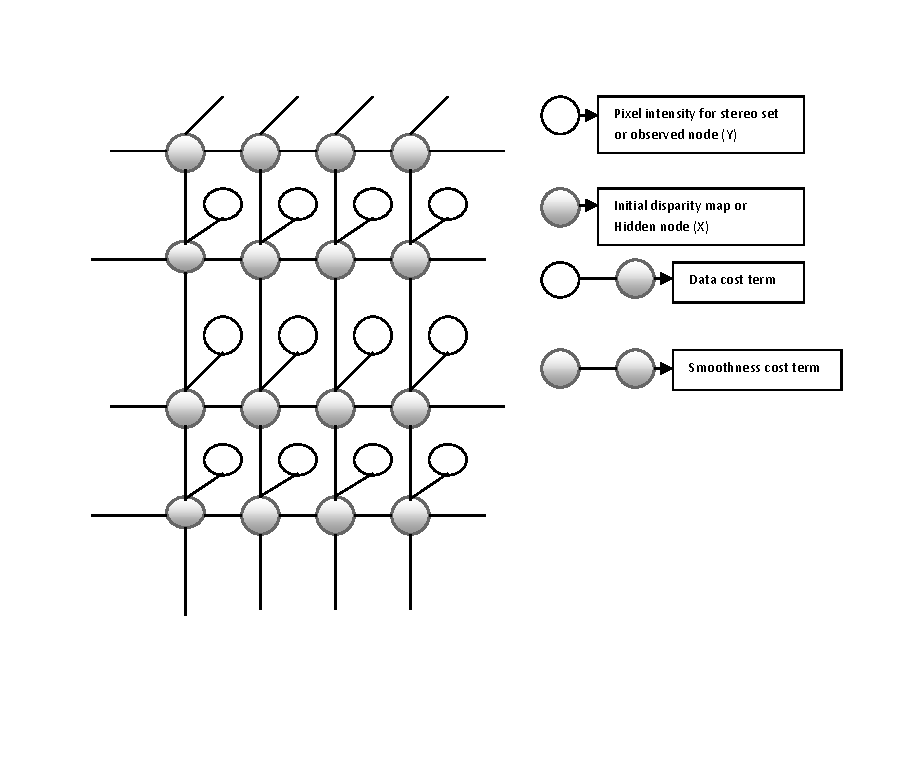
\includegraphics[width=5.5in]{markov.eps}
\caption{Stereo matching problem in Markov Representation } \label{lined}
\end{center}
\end{figure}

\begin{table}[h]
\caption{Stereo matching problem as probability theory and markov network }
\centering
Comparison of probability theory and Markov network are mentioned in table
\begin{tabular}{|p{1in}|p{2in}||p{3in}|}
\hline
  % after \\: \hline or \cline{col1-col3} \cline{col4-col5} ...
S.No.&Probability Theory & Markov network \\
  \hline
1& Maximizing probability of disparity map to stereo set i.e. $P(X/Y)$
 & Maximizing joint probability distribution i.e.
$P(X_1 ,X_2,�..X_n/Y)$ \\
\hline
 2& Set of pixels in disparity map each with assigned  disparity value
& Markov state \\
\hline
3&For given set of stereo images & For given Evidence Y \\
\hline
\end{tabular}
\label{table:comp}
\end{table}
Now stereo problem is reduce to finding Maximum A Posteriori (MAP) estimation in markov network.\newline To find Maximum A Posteriori (MAP) estimation in markov network is NP hard means to get a solution for such problem takes unthinkably long time which is because each pixel (node) in disparity map can take any value in disparity space (state).
\newline  Graph cuts and Belief Propagation are two global methods used to estimate Maximum a Posteriori (MAP) in reasonable amount of time
\section{Belief propagation}
The belief propagation algorithm was proposed by Pearl in 1988 for finding exact marginal's on graphs known as trees that contain no loops. The same concepts can be applied to the graphs which contains loops known as Loopy belief propagation.\newline The Loopy belief propagation is an approximate inference algorithm which keep passing the messages around markov state or node until stable belief state is reached, so the Loopy belief propagation algorithm is an iterative algorithm, messages will converge on doing iterations.\newline
There are three main steps finding Maximum a Posteriori (MAP) estimation or beliefs in markov network.
\begin{enumerate}
  \item 	Normalization
  \item 	Message update or generation
  \item  	Finding belief
\end{enumerate}
\begin{enumerate}
  \item \textbf{Normalization} is required because while continuously multiplying probabilities, messages becomes zero and hits the floating point limits. The normalization is difference of stereo set (observed node in markov network) to Initial disparity (hidden node in markov network) and divided by 256 for 8 bit brightness or gray level representation.
  \item \textbf{In Message updates or generation }step messages are updated by joint probability of data cost, smoothness cost and for all incoming messages which are marginalized over given disparity. Initially messages are updated or generated for right movement and similarly for up, left and for down movements. All these four movements of messages in message update step are in sum product approach. The Loopy belief propagation also known as Sum product algorithm.\newline
The final message in message update or generation step is a vector and size of the vector depends on disparity value.

  \item \textbf{In finding belief step,} the values of belief can be found either by Max Product belief propagation     or by Minimum of Sum belief propagation.
\end{enumerate}
\begin{figure}[h]
\begin{center}
\includegraphics[width=3.5in]{bp1.eps}
\caption{Flow chart for Belief Propagation } \label{lined}
\end{center}
\end{figure}



The best assignment of disparity can be assigned in maximum a posteriori (MAP) by finding largest marginal probability. The belief value in maximum a posteriori (MAP) at each node or state is maximum marginal.\newline
One of the important assumptions of Max Product belief propagation algorithm is belief values or maximum marginal values at each node or state are different. The belief values are converging by iterating Max Product belief propagation algorithm. The optimal assignment for maximum a posteriori (MAP) is depends on the number of iterations.




%\begin{tabular}{|Research paper|Optimization Method|Scope for Research|}
%  \hline
%  % after \\: \hline or \cline{col1-col2} \cline{col3-col4} ...
%   &  &  \\
%   &  &  \\
%   &  &  \\
%   &  &  \\
%  \hline
%\end{tabular}
%%

